\section{Konzeption einer an den spezifischen Workflow angepassten Anwendung}\label{l:konzeption}

Im Kapitel \ref{l:problemanalyse} wurde analysiert, welche Probleme in Zusammenhang mit der Produktion von Informations- und Kommunikationsmedien bezüglich den verwendeten Texten entstehen, wenn Textverarbeitungs- und Tabellenkalkulationsprogramme wie \trademark{Microsoft Word} und \trademark{Excel} verwendet werden. In diesem Kapitel wird eine Anwendung konzipiert, die den Anforderungen der im vorangegangenen Kapitel vorgestellten Personas entspricht und die beschriebenen Probleme beseitigt. Hierzu werden zunächst in Abschnitt \ref{l:workflow} und \ref{l:anforderungen} die Anforderungen beschrieben, bevor beginnend ab Abschnitt \ref{l:loesungsart} · S.\pageref{l:loesungsart} die Anwendung konzipiert wird, die diese Anforderungen erfüllt. 

\bigskip

In Kapitel \ref{l:entwurf} · S.\pageref{l:entwurf} wird auf Basis dieses Konzepts eine Anwendung entworfen und in Form eines Prototypen umgesetzt.

\subsection{Abzubildender Workflow}\label{l:workflow}

Hauptaufgabe der Anwendung ist es, den Workflow von der Definition bis zur Übernahme der fertigen Texte in das Produkt abzubilden und dabei nicht nur Funktionen zum \emph{Definieren}, \emph{Speichern} und \emph{Exportieren} zu bieten, sondern auch die \emph{Kommunikation über die Texte} zu integrieren. Für die Umsetzung des Workflows in einer Anwendung müssen zunächst alle Ausprägungen der speziellen Abläufe beschrieben werden. In Abschnitt \ref{l:besondererolle} wurde bereits gezeigt, wie umfangreich die Anzahl der Personen ist, die Einfluss auf die Texte eines Produkts haben. Die Rollenverteilung ist dabei von Projekt zu Projekt verschieden, mit den in Kapitel \ref{l:personas} vorgestellten Personas wurde eine Übersicht über die typische Rollenverteilung geschaffen. 

Betrachtet man die von Projektmitarbeitern durchgeführten Operationen in Zusammenhang mit Text lassen sich diese in sechs eigenständige Operationen unterteilen:

\begin{enumerate}
\item Durch \textbf{Definieren eines Textbausteines} werden dessen \emph{Attribute} bestimmt. Dadurch wird festgelegt, wie der benötigte Text beschaffen sein muss. Die Aussage \citequotes{Wir brauchen an dieser Stelle eine Überschrift} ist ein Beispiel für diese Operation. Sie legt fest, wie der Textbausteine gestaltet werden muss, um die ihm zugedachte Aufgabe zu erfüllen. Neben der Angabe zur Platzierung auf dem Medium durch \typoquotes{an dieser Stelle} wird implizit durch \typoquotes{eine Überschrift} eine Angabe zur inhaltlichen und visuellen Gestaltung getroffen; Überschriften sollen kurz und knapp sein und ihre visuelle Gestaltung wird durch den Styleguide des Projekts festgelegt.
\item Das \textbf{Schreiben eines Textes} erzeugt den Inhalt eines Textbausteins in einer Sprache. Bei diesem Vorgang wird der Text entsprechend der Vorgabe aus der Beschreibung als Original erstellt oder aus Quellen außerhalb des Projekts kopiert und eingefügt.
\item In der \textbf{Korrektur} wird der Text inhaltlich, orthografisch und grammatikalisch überprüft und entsprechend angepasst. Der Korrektor muss dabei für eine orthografische oder grammatikalische Überprüfung des Textes kein Fachwissen bezogen auf das Projekt haben. Ist diese Fachwissen vorhanden, kann eine inhaltliche Korrektur vorgenommen werden.
\item In der \textbf{Qualitätskontrolle} wird der Text dahingehend überprüft, ob er den Anforderungen gemäß der Beschreibung und inhaltlichen Vorgaben, auch hinsichtlich des gesamten Projekts entspricht.
\item Durch die \textbf{Freigabe} wird der Text abgenommen und kann nun in das Produkt übernommen werden. Die Freigabe unterscheidet sich von der Qualitätskontrolle durch ihren authorativen Charakter. Qualitätskontrollen können prinzipiell von allen Mitarbeitern durchgeführt werden. Freigaben werden nur von Mitarbeitern mit Management-Berechtigungen erteilt.
\item Durch die \textbf{Veröffentlichung} wird der Text in das finale Produkt eingebracht.
\end{enumerate}

\begin{samepage}
Verallgemeinert man diesen Ablauf, erkennt man, dass sich der Einfluss in vier grundlegende Eigenschaften der Texte unterteilen lässt:

\begin{enumerate}\itemsep -5pt
\item den \textbf{Inhalt} des Textes,
\item den \textbf{Vorgaben für diese Inhalte}
\item die \textbf{Attribute} wie z.B. \typoquotes{maximale Textlänge} oder \typoquotes{Position im Medium}
\item und den \textbf{Status} wie z.B. \typoquotes{neu} und \typoquotes{freigegeben}.
\end{enumerate}
\end{samepage}

Das Gewicht des Einfluss der Mitarbeiter ist je nach Rolle unterschiedlich, Tabelle \ref{table:texteinfluss} · S.\pageref{table:texteinfluss} zeigt dies in einer Übersicht.

\begin{table}
\begin{center}
\begin{tabular}{@{}r c c c c}
\textbf{Persona} & \textbf{Inhalt} & \textbf{Vorgaben} & \textbf{Attribute} & \textbf{Status}\\[1ex]
\textbf{Agentur} & & & \\
\hline\\[-1.5ex]
\emph{Eva}, Konzept & \HarveyHalf & \HarveyHalf & \HarveyFull & \HarveyEmpty \\
\emph{Lotte}, Art-Direktion & \HarveyEmpty & \HarveyEmpty & \HarveyThreeQuarters & \HarveyEmpty \\
\emph{Jan}, Produktion & \HarveyEmpty & \HarveyEmpty & \HarveyQuarter & \HarveyEmpty \\
\emph{Arthur}, Projektleitung & \HarveyEmpty & \HarveyQuarter & \HarveyEmpty & \HarveyQuarter \\[1ex]
\textbf{Extern} & & & \\
\hline\\[-1.5ex]
\emph{Torsten}, Text & \HarveyHalf & \HarveyQuarter & \HarveyEmpty & \HarveyEmpty \\
\emph{Jorinde}, Übersetzung & \HarveyQuarter & \HarveyEmpty & \HarveyEmpty & \HarveyEmpty \\[1ex]
\textbf{Kunde} & & & \\
\hline\\[-1.5ex]
\emph{Markus} & \HarveyHalf & \HarveyFull & \HarveyQuarter & \HarveyFull
\end{tabular}
\caption[Stärke des Einfluss, die Mitarbeiter in einem Projekt haben.]{Stärke des Einfluss, die Mitarbeiter in einem Projekt haben.\\\begin{tiny}{\HarveyEmpty} Kein Einfluss {\HarveyFull} Viel Einfluss\end{tiny}}
\label{table:texteinfluss}
\end{center}
\end{table}

\bigskip

Nachfolgend sind diese Text-Eigenschaften näher beschrieben.

\subsubsection{Inhalt}

Mit Inhalt ist der eigentliche Text gemeint, der auch im Produkt erscheint. Für Inhalte gibt es immer eine Original-Version für die im späteren Projektverlauf Übersetzungen in eine oder mehrere Sprachen angelegt werden können. Die Übersetzung basiert dabei auf der Original-Version, oder je nach Übersetzer auch auf einer anderen Übersetzung.

Personen die Einfluss auf den \emph{Inhalt} haben, sind vor allem diejenigen die die Texte für das Produkt liefern. Dies sind vor allem Texter und Übersetzer. Üblich sind aber auch Anpassungen der Inhalte durch Experten. Ein Beispiel hierfür ist die Suchmaschinenoptimierung von Texten. Hierbei werden Texte auf das Vorhandensein von bestimmten Formulierungen und Stichwörtern hin optimiert. 

\subsubsection{Inhaltsvorgaben}

Vorgaben für Inhalte sind werden in Form von Richtlinien formuliert und nicht ins Produkt übernommen. Diese Richlinen dienen Textern als Orientierungshilfe, wie die Texte zu formulieren sind. Richtlinien werden von verschiedenen Mitarbeitern formuliert: 
\begin{itemize}\itemsep -5pt
\item Vom Konzept werden grundlegende Vorgaben geschaffen, wie z.B. Annahmen über die Zielgruppe und den Zweck des Produkts.
\item Der Kunde hat Vorstellungen oder sogar Vorgaben, wie der Sprach-Stil der Texte sein soll, aus seinen Fachabteilungen und von Beratern oder Anwälten werden weitere Vorgaben über erwünschte oder zu vermeidende Aussagen erstellt.
\item Nicht selten werden externe Experten zu Projekten hinzugezogen, die für bestimmte Aspekte Richtlinien definieren. Besonders bei Internetseiten werden SEO-Konzepte erstellt, die festlegen, dass die Texte bestimmte Schlüsselwörter und Formulierungen enthalten sollen, um in den Algorithmen der Suchmaschinenbetreiber bessere Positionierungen in Suchergebnissen zu erreichen.
\end{itemize}
Es existieren aber auch implizite Vorgaben, die sich aus der Art des Mediums ergeben: Lange Texte sind für Fernsehspots ungeeignet, Informationsbroschüren haben Raum für ausführliche Erläuterungen. Diese impliziten Vorgaben müssen ebenfalls explizit hinterlegt werden, um möglichst wenig Raum für Interpretationen durch die Autoren der Texte zu bieten.

% MARK

\subsubsection{Attribute} 

Attribute legen die Rahmenbedingungen von Text fest, diese werden vor allem in der Gestaltung des Produkts durch Designer, als auch in der Umsetzung durch produktbedingte Einschränkungen, z.B. Platzverhältnisse oder systembedingte Beschränkungen, bestimmt. Attribute sind in irgendeiner Form quantifizierbare Angaben zu Textbausteinen. Sie dienen zum einen dazu, den Textbaustein zu identifizieren und seine Rolle im Produkt festzulegen und zum anderen werden damit Vorgaben zur Beschaffenheit des Textes festgelegt. Die Attribute lassen sich in vier Bereiche unterteilen:

\paragraph{Identifier} Dies sind eindeutige Bezeichner für Textbausteine, diese dienen dazu, Referenzen zwischen den Textbausteinen in der Anwendung und im Produkt herzustellen, z.B. um automatische Aktualisierungen zu ermöglichen. Identifier werden auch benötigt, damit Kommentare, Zusatzinformationen usw. diesen eindeutig zugordnet werden können.

\paragraph{Klasse} generell lassen sich die Texte in jedem Produkt in wenige, deutlich unterscheidbare Klassen unterteilen. Aus Gründen der Usability versucht man bei der Gestaltung von Medien ein einheitliches Gestaltungsbild zu erreichen, dazu gehört auch, dass Texte, die die gleiche Funktion haben, auch gleich gestaltet werden. In den meisten Fällen gibt es eine Unterscheidung zwischen Fließtext und Überschriften, die es auf mehreren Hierarchieebenen gibt. Bei interaktiven Produkten finden sich dann häufig Texte für Navigations-Elemente wie Buttons und Links oder für die Verwendung in Formularen. Bei der Klassifizierung von Texten werden die Schriftart, Schriftgröße, Schreibweise  (z.B. nur GROSSBUCHSTABEN) und weitere Angaben zu Formatierung (z.B. Abstände zum nächsten Textbaustein) bestimmt, die für alle Texte dieser Klasse verwendet werden. Zusätzlich werden üblichweise auch noch weitere Regeln für die Verwendung der Klassen festgelegt, z.B. dass auf eine Headline immer vor einem Fließtext stehen muss. Teil der Klassifizierung können auch Angaben zur Zeichenlänge enthalten, da dies aber nicht immer zwingend der Fall ist und es auch Textlängenbeschränkungen ohne Bezug zur Klasse eines Textes geben kann (z.B. bei Forumularen) werden diese separat betrachtet.

\paragraph{Textlänge} In vielen Fällen ist es aus gestalterischer, inhaltlicher oder technisches Sicht gewünscht, dass die Textlänge eines Textbausteines in einem gewissen Rahmen liegt. Üblich sind Vorgaben zur minimalen, maximalen und gewünschten Anzahl von Zeichen, Wörtern, Sätzen, Zeilen und Absätzen

\paragraph{Position} Zu jedem Textbaustein wird festgelegt, wo dieser im Produkt erscheint. Diese Information ist besonders für die Produktion wichtig, aber auch schon vorher wird diese Information immer wieder benötigt, z.B. um vor Fertigstellung des Produkts eine Vorschau oder einen Dummy einzelner Bestandteile des Produkts anzufertigen. Positionsangaben bestehen meistens aus zwei Komponenten. Zum einen wird eine hierarchische Position definiert, z.B. auf \citequotes{im zweiten Kapitel}, oder \citequotes{unter der Überschrift auf der Seite \typoquotes{Über uns}.} Zum anderen kann es exakte Postionsangaben und Größenangaben geben. Diese haben zwar keinen direkten Einfluss auf den Text, können aber für Produkte mit festen Gestaltungsrahmen und den Informationen zur Textklasse wichtige Hinweise darüber liefern, wie lang der Text maximal sein darf, ohne das Layout \typoquotes{zu sprengen}.

\subsubsection{Status}\label{l:konzept-workflow-status}

Den Status von Texten, also ob ein Text dem nächsten Mitarbeiter im Workflow zugewiesen werden soll kann von bestimmten Mitarbeitern abhängen. Es ist üblich, dass Texte erst dann dem Kunden zur Abnahme vorgelegt werden, wenn sie als Gesamtes vorliegen. Auch externe Dienstleister bekommen aus Kostengründen meisten alle Text im Paket, damit eine zügige Abarbeitung des Auftrages gewährleistet wird. Praktisch ist der Status eines Textes dem aktuellen Bearbeiter gleich zu setzen. Eine Änderung des Status bedeutet, dass der aktuelle Bearbeiter seine Aufgabe abgeschlossen hat und der nächste Bearbeiter mit seiner Aufgabe weitermachen kann. Es kann auch eine Statusänderung in umgekehrter Richtung geben, wenn der die Vorbedingungen für den nächsten Mitarbeiter nicht erfüllt sind, oder bei einer Kontrolle ein Problem festgestellt wird. Je nach Mitarbeiter unterscheidet sich, zu welchen Zeitpunkt und zu welchen Status er Feedback gibt. Abbildung~\ref{chart:workflowmitfeedback} · S.\pageref{chart:workflowmitfeedback} gibt einen Überblick über die Entscheidungsprozesse im Verlauf eines Projekts und wer auf diese Einfluss nimmt. Tabelle \ref{table:workflowmitfeedback} · S.\pageref{table:workflowmitfeedback} listet den Einfluss tabellarische und enthält zusätzlich Informationen, wie stark der jeweils ausgeübte Einfluss in der Regel ist.

\begin{figure}[htb]
\begin{center}
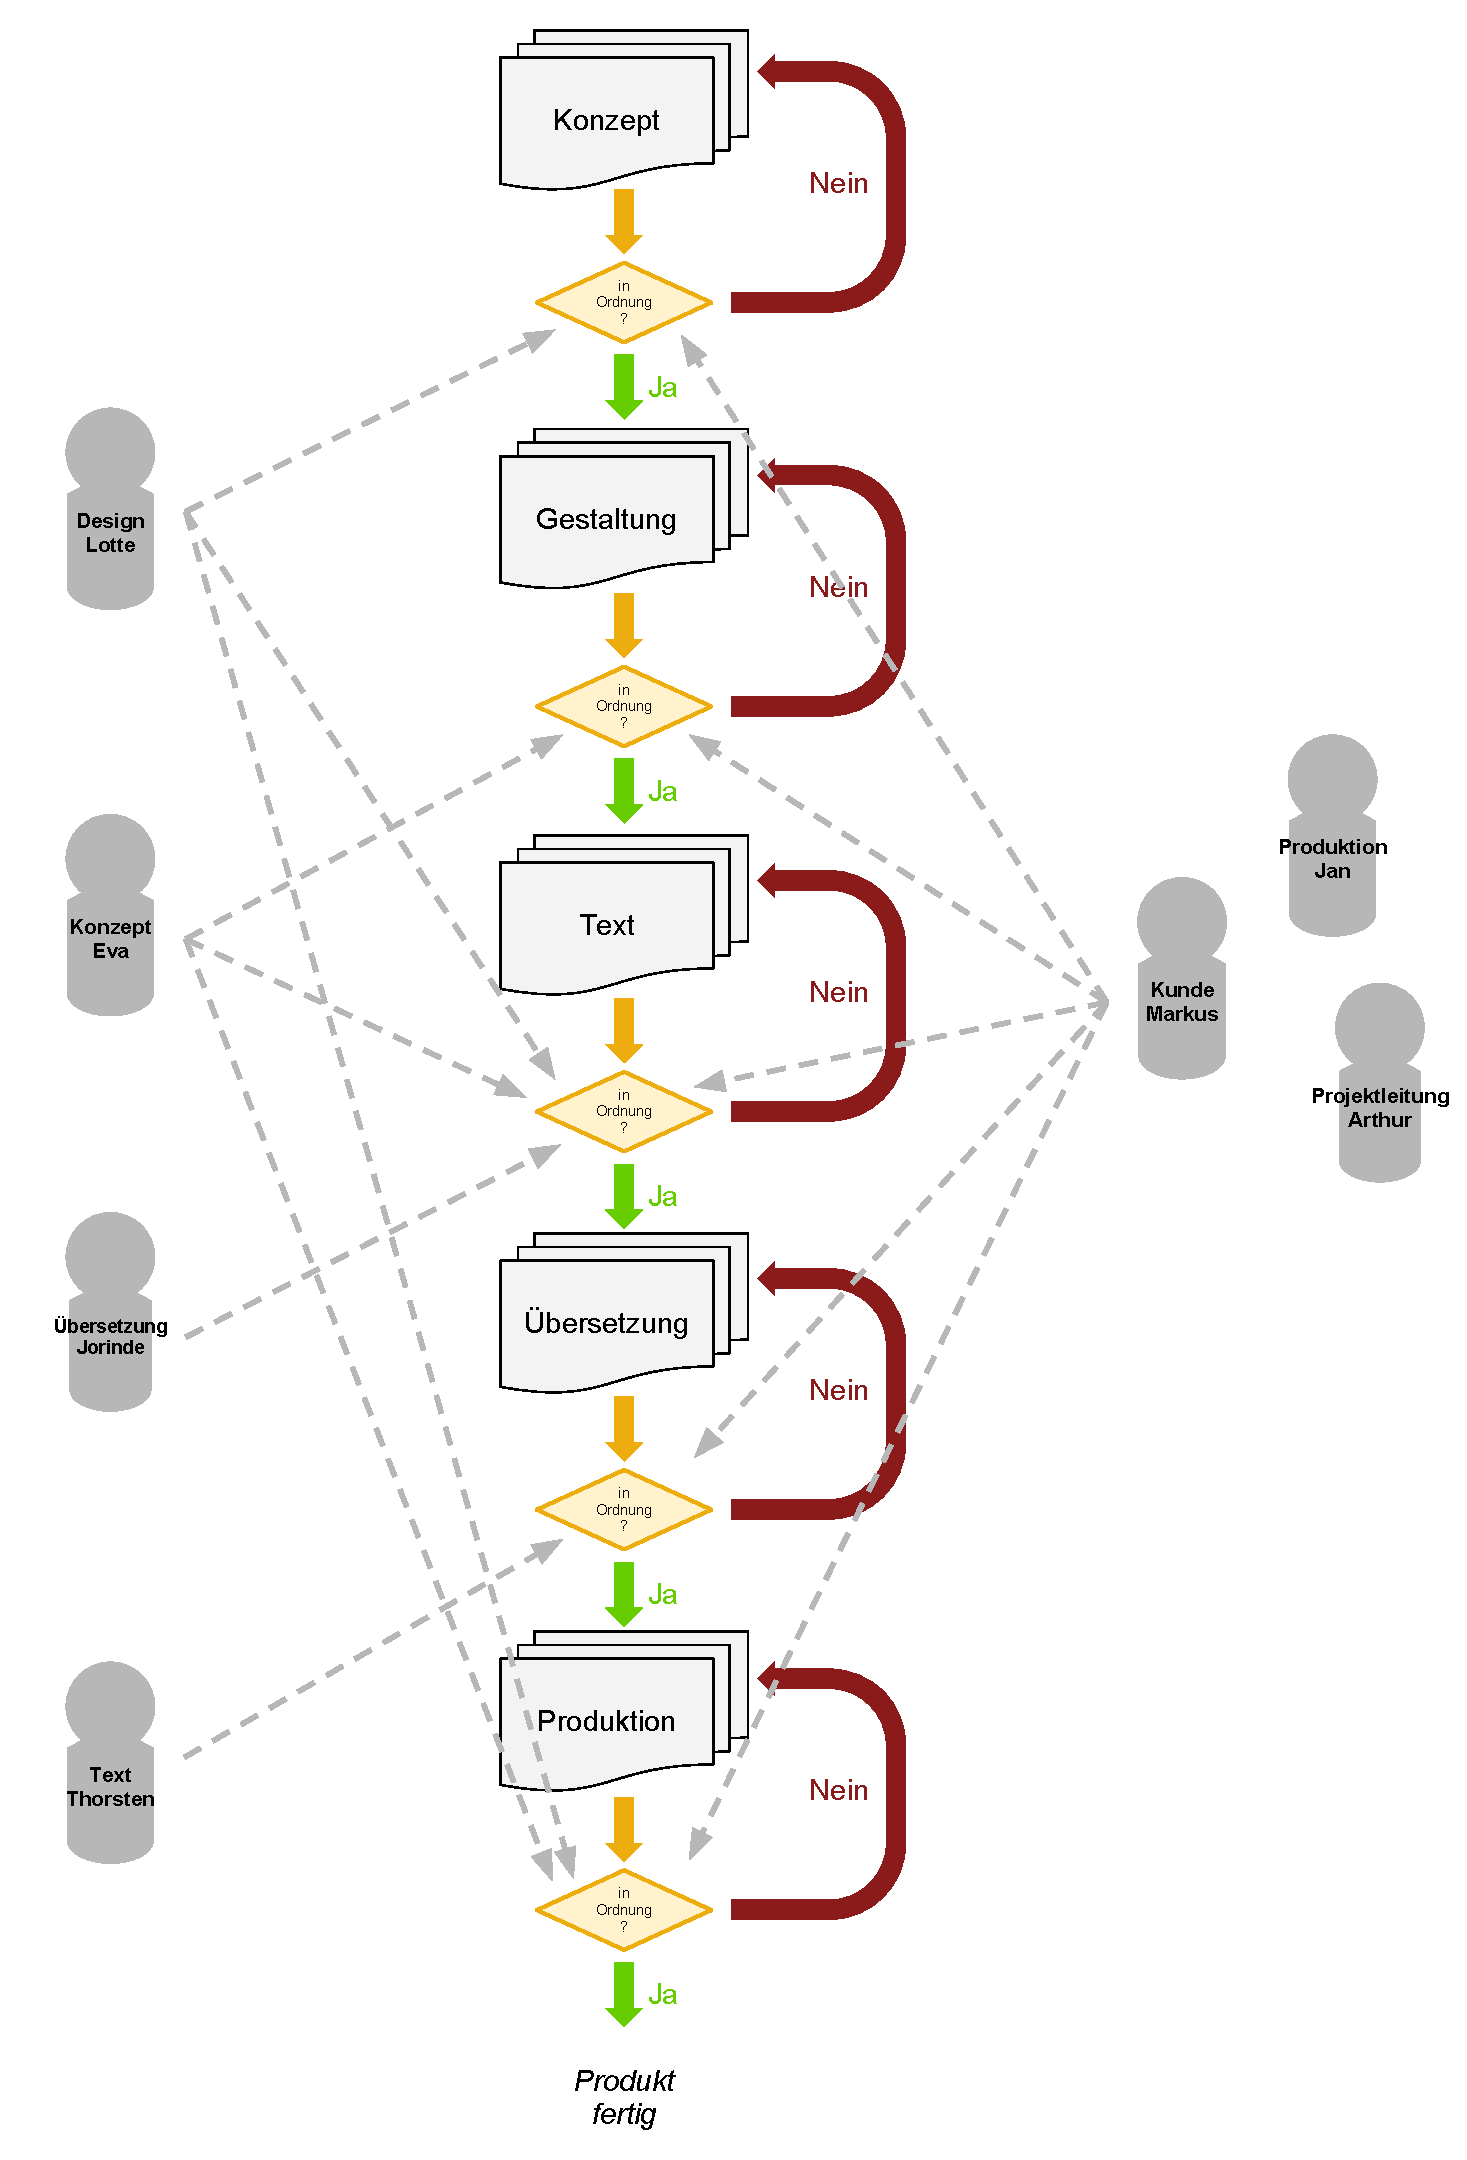
\includegraphics[width=0.6\textwidth]{media/WorkflowmitFeedback.pdf}
\end{center}
\caption{Einfluss auf den Status eines Textbausteines}
\label{chart:workflowmitfeedback}
\end{figure}

\begin{table}
\begin{center}
\begin{tabular}{@{}l c c c c c c c}
& \textbf{Eva} & \textbf{Lotte} & \textbf{Torsten} &  \textbf{Jorinde} & \textbf{Jan} & \textbf{Arthur} & \textbf{Markus}\\
{\small Einfluss auf} & {\small Konz.} & {\small Des.} & {\small Texter} & {\small Übersetz.} & {\small Prod.} & {\small Projektl.} & {\small Kunde}\\
\hline\\[-1.5ex]
Konzept & \HarveyFull & \HarveyQuarter & \HarveyEmpty & \HarveyEmpty & \HarveyQuarter & \HarveyHalf & \HarveyThreeQuarters \\
Design & \HarveyQuarter & \HarveyFull & \HarveyEmpty & \HarveyEmpty & \HarveyQuarter & \HarveyQuarter & \HarveyThreeQuarters \\
Text & \HarveyHalf & \HarveyQuarter & \HarveyFull & \HarveyQuarter & \HarveyQuarter & \HarveyQuarter & \HarveyHalf \\
Übersetzung & \HarveyEmpty & \HarveyEmpty & \HarveyHalf & \HarveyFull & \HarveyQuarter & \HarveyQuarter & \HarveyHalf \\
Produktion & \HarveyHalf & \HarveyHalf & \HarveyEmpty & \HarveyEmpty & \HarveyFull & \HarveyHalf & \HarveyFull \\
\end{tabular}
\caption{Einfluss mit Gewichtung auf den Status eines Textbausteines}
\label{table:workflowmitfeedback}
\end{center}
\end{table}

\paragraph{Ereignisse} Da sich die Texte des Produkts aus vielen einzelnen Bausteinen zusammensetzen, werden auch die Eigenschaften jeweils einzelnen gesetzt. Aus Sicht des Projektverlaufes ergeben sich aus der Gesamtheit alle Zustände bestimmte Ereignisse, die sich auf die Änderung der Stati der Texte zurückführen lassen. Immer dann, wenn alle Texte eines Produkts einen gewissen Status erreichen, werden bestimmte Ereignisse ausgelöst. Ein Beispiel: erst wenn alle Texte durch den Kunden abgenommen wurden, werden diese an die Übersetzung übergeben. Dies stellt sicher, dass die Übersetzung nur die Texte übersetzt, die auch benötigt werden und somit keine unnötigen Kosten verursacht.

\pagebreak

\subsection{Anforderungen an die Anwendung}\label{l:anforderungen}

Neben den im vorangegangenen Abschnitt beschriebenen Anforderungen an den Workflow, muss die Anwendung weitere Eigenschaften erfüllen. Die wichtigsten werden nachfolgend kurz beschrieben.

\paragraph{Gleichzeitiges Bearbeiten}

Es ist essentiell, die Beschränkungen eines seriellen Bearbeitungskonzeptes, wie es durch \trademark{Word} und \trademark{Excel} vorgegeben wird, aufzuheben und das gleichzeitige Bearbeiten der Inhalte des Projekts zu ermöglichen. 

\paragraph{Benutzerverwaltung und Nachvollziehbarkeit}

Die Abbildung eines Workflows setzt voraus, dass die Beteiligten am Projekt eindeutig identifiziert werden können und dass es möglich ist, die Aufgaben explizit zu verteilen. Das ist auch Voraussetzung für eine weitere Anforderungen nach der Nachvollziehbarkeit aller Änderungen.

\paragraph{Zugang von überall}

Da sich die Projektbeteiligten nicht alle an einem Ort befinden, muss der Zugang zur Anwendung über das Internet möglich sein.

\paragraph{Zugriff von verschiedenen Plattformen}

Es gibt unterschiedliche Anforderungen an den Zugang zur Plattform, dieser muss möglichst von vielen Endgeräten und dabei sowohl von stationären Systemen als auch von unterwegs aus möglich sein.

\paragraph{Integration in die Werkzeuge}

Für viele Arbeiten in Zusammenhang mit der Erstellung von Medien werden spezialisiert Werkzeuge verwendet, die durch die hier vorgestellte Lösung niemals ersetzt werden können. Es muss also eine Integration in diese Werkzeuge mit Hilfe von Plug-Ins oder ähnlichem existieren, mit denen es möglich wird, die Texte aus der Anwendung in die Produkte zu übernehmen. Zur Anbindung dieser Plug-Ins wird eine Schnittstelle (API) benötigt.

\paragraph{Umfangreiche Export-Funktionen}

Um die Texte in das Produkt zu integrieren, bedarf es umfangreicher Exportfunktionen in strukturierete Formate wie z.B. XML. Zur Kontrolle oder um eine Übersicht über das Produkt zu bekommen ist es erforderlich den Export in Dokumentenformate wie \trademark{PDF} und \trademark{Word} zu ermöglichen.

\pagebreak

\subsection{Art der Anwendung}\label{l:loesungsart}

Die im vorangegenen Abschnitt beschriebenen Anforderungen an die Anwendung, besonders im Hinblick auf den universellen, jederzeitigen Zugriff von überall sind die entscheidenden Anforderungen, die für die konzeption der Anwendung als \emph{browserbasierte Web-Anwendung mit vollständiger Schnittstellen-Abdeckung} sprechen. 

\bigskip

\begin{figure}[htb]
\begin{center}
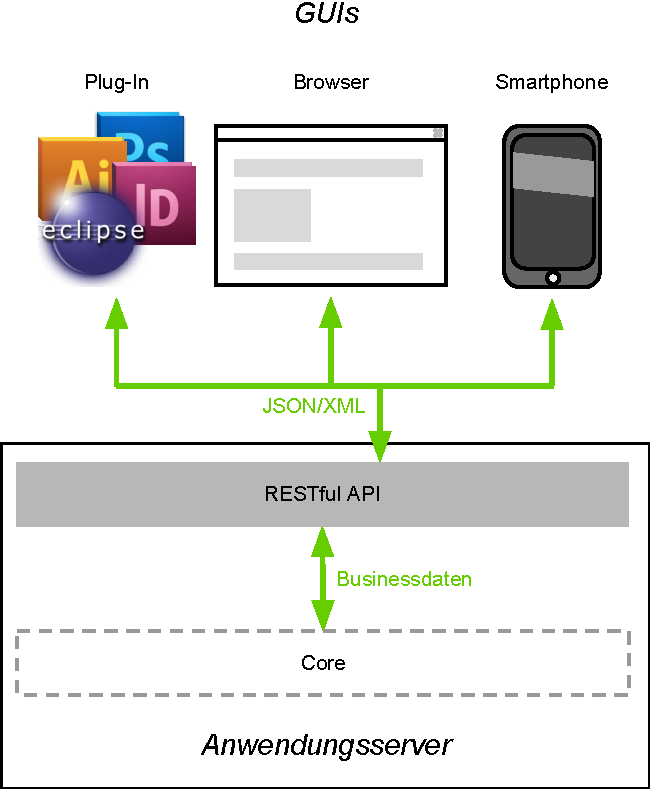
\includegraphics[width=0.65\textwidth]{media/ArtdesSystems.pdf}
\caption{Aufbau der Anwendung in stark vereinfachter Darstellung}
\label{chart:aufbaudessystems}
\end{center}
\end{figure}

Diese Klasse von Anwendung verwendet einen Webbrowser als Laufzeitumgebung. Dabei stellt der Browser das GUI der Anwendung mit Hilfe von HTML, CSS und JavaScript dar, die Businesslogik und die Datenhaltung wird auf einem Server ausgeführt, mit der das GUI mithilfe einer Schnittstelle kommuniziert. Abbildung~\ref{chart:aufbaudessystems} · S.\pageref{chart:aufbaudessystems} zeigt den Aufbau der Anwendung in stark vereinfachter Darstellung. War es in den letzten Jahren noch üblich, dass Fragmente des GUIs mit serverseitigen Template-Sprachen erzeugt wurden (vgl.~\cite[S.48]{dunkel2008systemarchitekturen}) hat die zunehmende Verbreitung von mobilen Clients ein Umdenken zur Folge. Zum einen stellen Desktop-Clients, mobile Browser-Clients und native Apps zwar die gleichen Daten einer Anwendung dar, verwenden dafür aber nicht zwangsläufig die gleiche GUI-Technologie. Zum anderen werden Clients immer leistungsstärker, selbst Einsteiger-Smartphones haben inzwischen CPUs mit mindestens dreistelligem Megahertz-Wert. Diese Entwicklung führt gerade bei Web-Anwendungen, auch Rich Internet Applications (RIAs) genannt, zu der Idee, Architekturen zu entwickeln, bei denen serverseitig keine GUI-Komponenten mehr erzeugt werden (vgl.~\cite{maccaw2011javascript} und \cite{coates2012phptemplating}). Clients kommunizieren über Schnittstellen mit dem Server und tauschen nur noch reine Daten aus. Dies hat mehrere Vorteile. Zum einen muss serverseitig kein Modell der clientseitigen Darstellung verwaltet werden, zum anderen verkleinert sich die Menge der transferierten Daten zwischen Client und Server erheblich. Dies hat besonders bei Benutzern mit langsamen oder schlechten Datenverbindungen im Mo"-bil"-funk-Netz große Vorteile. Für Web-Anwendungen bedeutet dass diese das zur Darstellung benötigte HTML mit Hilfe von JavaScript selber direkt im Client erzeugen. Beim ersten Besuch einer Internetseite müssen lediglich einmal die JavaScript-Dateien und benötigte statische Ressourcen wie CSS-Dateien, Bilder und ein statischer HTML-Grundaufbau geladen werden. Anschließend werden nur noch die für die jeweilige Aktion benötigten Daten mit Hilfe von JavaScript zwischen der Anwendung und dem Server ausgetauscht. Mobile Endgeräte, die über eigene GUI-Toolkits verfügen, oder Software von Drittanbietern können dann die selben Schnittstellen verwenden, ohne dass serverseitige Anpassungen vorgenommen werden müssen.

Web-Anwendung haben den Vorteil, dass sie ohne Installation auf dem Rechner des Benutzers lauffähig sind. Sie können als unmittelbar verwendet werden. Kompaitibilätsprobleme mit alten Browser-Versionen (z.B. dem \trademark{Internet Explorer 6}) können inzwischen mit Hilfe des \trademark{ChromeFrame}\footnote{\url{https://developers.google.com/chrome/chrome-frame/}} komfortable umgangen werden. Der Umfang an frei verfügbaren Bibliotheken zur Erstellung attraktiver und angenehm benutzbarer Anwendungen auf Basis von HTML ist riesig. Web-Anwendungen können mit wenig Aufwand auch auf mobilen Endgeräten eingesetzt werden, da Technologien zur platformabhängigen Anpassung der Darstellung (z.B. CSS-Mediaqueries) existierten. Insgesamt sind Webbrowser der aktuellen Generation mächtige Werkzeuge zur Erstellung von CRUD-Anwendungen. \cite{ms-key-software-development-trends} Die allgemeinen Vorteile einer browserbasierten Software, auch als \emph{Software as as Service} (SaaS) oder \emph{Application Service Provider} (ASP) Modell bekannt, liegen auf der Hand und werden an dieser Stelle nicht detailliert ausgeführt. Um nur einen zu nennen: die Möglichkeit, die Software jederzeit und für alle Mitarbeiter gleichzeitg ohne deren Zutun aktualisieren zu können, eliminiert vielfältige Probleme, die sonst in Umgebungen entstehen, in denen unterschiedliche Programmversionen existieren.

\pagebreak

\subsection{Schnittstellen} 

Die Verwenden einer einheitlichen Schnittstelle durch alle Clients ermöglicht ein konsistentes Verhalten der Anwendungen über alle Zugangswege hinweg und ist besonders in Fall dieser Anwendung von Bedeutung, da die Benutzer wünschen, dass sich die Texte direkt innerhalb ihrer bevorzugten Werkzeuge abrufen und einbinden lassen. Dies ist nur mit Hilfe von Plugin-Ins möglich, die in der jeweiligen Umgebung der Software entwickelt werden müssen. Aus diesem Grund ist es ungvermeidlich, dass für alle Funktionen der Anwendung eine öffentliche Schnittstelle existiert.

Als Protokoll zur Kommunikation zwischen Clients und Server hat sich REST bewährt. Die Struktur des Protokolls ist direkt mit dem HTTP-Protokoll vebunden, so ist die Verarbeitung von REST-Anfragen serverseitig leicht mit Web-Frameworks zu implementieren, da diese von sich aus bereits für diese Art von Anfragen ausgelegt sind. Clientseitig wird lediglich ein HTTP-Client benötigt sowie Module zum Parsen von JSON- oder XML-Da"-ten"-struk"-tu"-ren -- Voraussetzungen, die von Browsern und Smartphones erfüllt werden. JSON hat im Vergleich zu SOAP den Vorteil, dass es nicht versucht die Architektur der zugrundeliegenden Software nach außen abzubilden, so muss sich der Client nicht an bestimmte Reihenfolgen im Aufruf von Methoden halten. In der REST-Welt sind alle Operationen atomar und können ohne Vorbedingung gestellt werden. In der Praxis ist dies nicht immer umsetzbar, REST fordert serverseitig Zustandslosigkeit, die aber bei Anwendungen in denen Daten gespeichert und verändert werden nicht realisierbar ist. Aufgrund seines flexibleren Aufbaus, der Möglichkeit ausgewählte Anfragen leicht mit HTTP-Caches zu beschleunigen und der freien Wahl der Nachrichtenformats ist REST aus Sicht des Autors die besser Wahl zur Implementierung der Schnittstellenkommunikation.

\pagebreak

\subsection{Zugang}

Diese Konzeption macht es möglich, jedem Mitarbeiter den passenden Zugang zu ermöglichen, im Einzelnen sind das:

\paragraph{Browserbasierter Zugang vom Desktop} Den Webbrowser werden alle Mitarbeiter verwenden, da in diesem GUI alle Funktionen der Anwendung implementiert sind.

\paragraph{Browserbasierter Zugang von Smartphones} Auf gängigen Smartphones sind Browser vorhanden, die in der Lage sind, die selben Inhalten anzuzeigen, wie ihr Desktop-Equivalent. Aufgrund der deutlich kleineren Bildschirmgröße und dem fehlen einer Maus ist es aber sinnvoll, dem Rechnung zu tragen und eine angepasste Version der Anwendung für diese Geräte bereit zustellen. 

\paragraph{Zugang direkt über die Schnittstellen} Vor allem im Bereich der Software-Entwicklung wird der direkte Zugriff der Entwickler auf die Schnittstellen der Anwendung eine wichtige Rolle spielen. So können diese die Integration der Anwendung in ihren Entwicklungsprozess optimal an die jeweiligen Bedürfnisse anpassen.

\paragraph{Exporte} Die Möglichlichkeit, die Texte des Projekts in verschiedene Formate zu exportieren ist eine wichtige Funktion. Sie ermöglicht zum einen die Übernahme in Systeme und Anwendungen, deren Anbindung nicht möglich oder gewünscht ist und schafft zum anderen die Möglichkeit, ähnlich wie Schnittstellen, die verarbeiteten Daten auf eine Art und Weise zu verwenden, die nicht vorhergesehen wurde oder nicht im Sinne der Anwendung liegt.

\paragraph{Zugang über Plug-Ins} Besonders für Mitarbeiter in der Produktion kann es wichtig sein, auf ihre angestammten Werkzeuge nicht verzichten zu müssen. Plug-Ins, also Erweiterungen für diese Werkzeuge, integrieren dann Teile der Funktionen der Anwendung in diese Werkzeuge. Beispielsweise könnte es ein Plug-In für \trademark{Adobe InDesign} ermöglichen, auf die Texte aus der Anwendung zuzugreifen und diese direkt in Text-Rahmen im \trademark{InDesign}-Dokument zu übernehmen, so dass Copy\&Paste der Texte aus der Web-Anwendung oder einem exportierten Dokument entfallen kann.

\paragraph{Benachrichtigungen} Benachrichtigungen sind eine Form des Zugangs, die es Benutzern der Anwendung ermöglicht, über bestimmte Ereignisse informiert zu werden. Benachrichtigungen können in Form von E-Mails, SMS, über soziale Netzwerke wie Twitter, über Chat-Dienste wie Skype, IRC statt finden. Hierbei werden Information zu einem Ereignis übertragen z.B. der Status-Änderungen eines Textes. Denkbar sind auch auch Push-Exporte der Texte aufgrund eines bestimmten Ereignisses, z.B. der FTP-Export der Texte als CSV-Datei, sobald das Projekt abgschlossen ist oder Änderungen freigegeben wurden.

\paragraph{Software von Drittanbietern} Dadurch, dass alle Funktionen der Anwendung über eine Api exponiert werden, sind auch fremde Softwarehersteller in der Lage, Teile der Funktionen oder die gesamte Anwendung in einer eigenen GUI zu implementieren. So können Bedürfnisse von Anwendergruppen mit besonderen Anforderungen abgedeckt werden, die bei der Konzipierung der Anwendung nicht berücksichtigt wurden.

\pagebreak

\subsection{Überblick über den Aufbau der gesamten Anwendung}

Abbildung~\ref{chart:gesamtessystem} liefert einen Überblick über den Aufbau der gesamten Anwendung:

\begin{figure}[htb]
\begin{center}
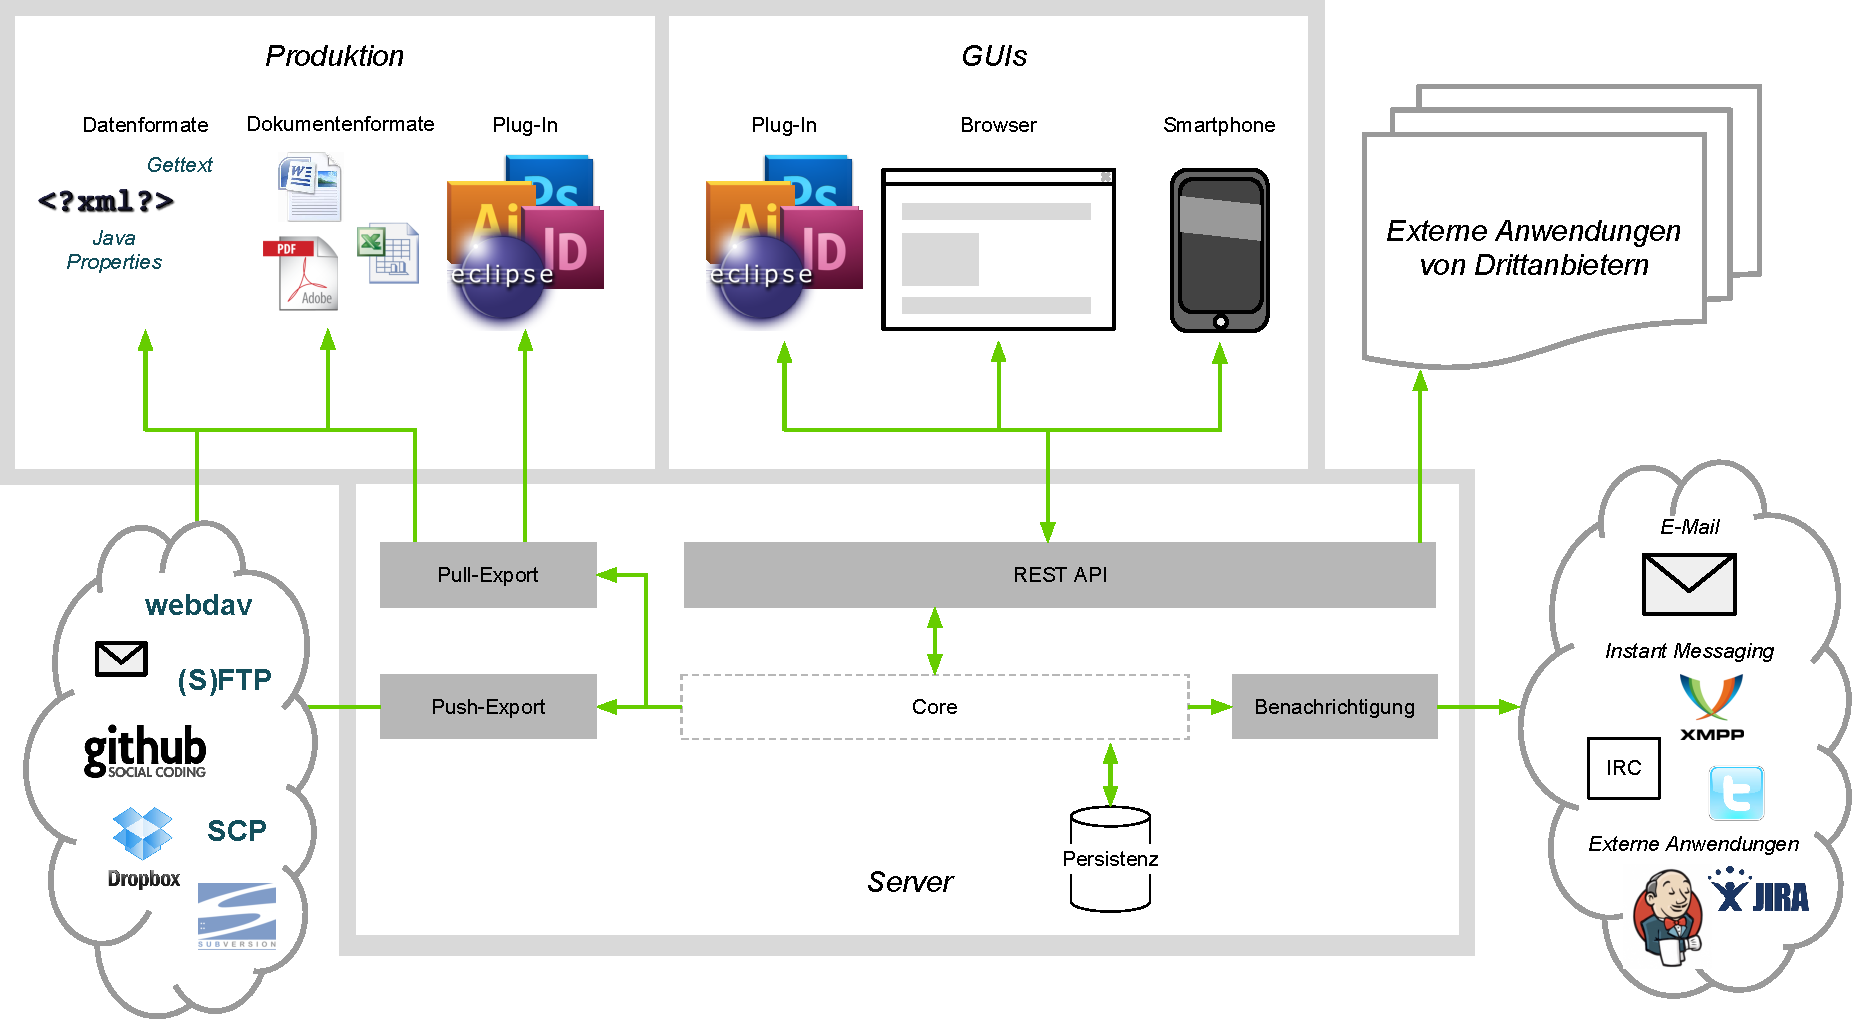
\includegraphics[width=\textwidth]{media/GesamtesSystem.pdf}
\caption{Aufbau der gesamten Anwendung im Überblick}
\label{chart:gesamtessystem}
\end{center}
\end{figure}

Die Zentrale Komponente der Anwendung bildet der Server. Für die Benutzer erfolgt der Zugriff mit Hilfe einer GUI, die mit der REST-API des Servers kommuniziert. Eine browserbasierte GUI auf Basis von HTML5 und JavaScript bildet den Hauptzugang zur Anwendung, der auch auf Smartphones verwendet werden kann. Zusätzlich gibt es spezielle Plugins für Adobe-Produkte und weitere wichtige Produktionsumgebungen. Auch native GUIs für Smartphones verwenden die gleiche API. Die Schnittstellen können auch von Drittanbietern dazu verwendet werden, eigenen Clients für die Anwendung zu entwickeln. In die Endprodukte gelangen die Texten über den Export, exportiert wird dabei in viele Formate, neben Datenformaten wie z.B. XML werden auch Dokumentenformate wie z.B. Word exportiert. Der Export kann durch den Anwender erzeugt werden (\emph{Pull-Export}), aber auch automatisch, z.B. nach festgelegten Zeitplänen oder Ereignissen erfolgen. Dieser \emph{Push-Export} erfolgt auf je nach Projekt festlegbaren Orte, wie z.B. FTP-Server oder Versionsverwaltungssysteme. Die Benachrichtigungen über Aufgaben und Änderungen an Texten kann via E-Mail, aber auch mittels Instant-Messaging-Systeme oder durch den Aufruf fremde API-Endpunkte erfolgen.

\pagebreak

\subsection{Zusammenfassung, Nachteile \& Risiken des Konzepts}

In diesem Kapitel wurde eine Anwendung konzipiert und der darin abgebildetet Workflow beschrieben. Die Konzipierung der Anwendung als Web-Anwendung, bei der alle durchführbaren Operationen über Schnittstellen abgedeckt sind, ermöglicht es, für jeden Mitarbeiter die passenden Zugangswege anzubieten. Als Hauptzugang wird der Webbrowser verwendet, so ist sichergestellt, dass alle Mitarbeiter alle Funktionen der Anwendung ohne zusätzliche Aufwände wie die Installation neuer Software verwenden können. Für spezielle Anwendungsfällen ist es mit Hilfe der API möglich, Plug-Ins zu entwickeln, die sich in die bevorzugten Werkzeuge der Anwender integrieren.

\paragraph{Nachteile \& Risiken} Ein Nachteil dieses Konzepts liegt in der Zentralisierung der Datenspeicherung. Da alle Daten auf einem zentralen Server verwaltet werden, ist dieser auch der \emph{Single Point of Failure}, d.h. sollte der Server ausfallen, kann kein Mitarbeiter weiterarbeiten. Für einen kommerziellen Betrieb einer solchen Anwendung ist es also unabdingbar, dass die Server-Infrastruktur ausfallsicher konzipiert ist. 

Das Übertragen der Daten auf einen zentralen Server kann auch zu Bedenken bei den beteiligten Unternehmen führen. Es gibt gerade bei größeren Unternehmen Vorbehalte dagegen, Informationen auf Systemen von Drittanbietern zu speichern. Hier gilt es, genau wie im Hinblick auf die Verfügbarkeit der Anwendung, einen vertrauenswürdigen Betreiber für die Server-Infrastruktur zu finden. Alternativ ist es jedoch problemlos möglich, die Anwendung auch \emph{In-House}, also auf Servern im Unternehmen als \emph{Appliance}, zu betreiben, wobei dann aber zusätzliche Wartungsaufwände entstehen, und damit einige Vorteile des SaaS-Modells ausgehebelt werden. 

Da alle Mitarbeiter über das Internet mit der Anwendung verbunden sind, spielt auch die Bandbreite und Verfügbarkeit einer Internetverbindung eine Rolle. Im Unternehmensbereich spielt dies aber inzwischen nur nur eine untergeordnete Rolle. Trotzdem sollten geeignete Maßnahmen ergriffen werden, die die Arbeit auch mit einer langsamen oder sogar ganz ohne eine Internetverbindung ermöglicht (Offline-Access).

Das größte Risiko dieses Konzeptes ist, dass Mitarbeiter gezwungen werden, sich von ihren bekannten Werkzeugen zu lösen. Gerade bei Mitarbeitern, die vor allem mit Textverarbeitungsprogrammen arbeiten und ansonsten kaum mit anderen Werkzeugen Kontakt haben, wird der Umstieg von der unstrukturierten Arbeitsweise in \trademark{Word} auf die, bis auf den einzelnen Text heruntergebrochene Arbeitsweise in der vorgschlagenen Anwendung, schwer fallen. Man kann aber davon ausgehen, dass für alle Beteiligten die Vorteile der Lösung erkenntlich werden und sich eine Abneigung gegen eine Änderung angestammter Arbeitsabläufe leicht abbauen lässt.

\secbar

Im nächsten Kapitel wird eine Anwendung entworfen, die dieses Konzept umsetzt.

\pagebreak